\begin{tikzpicture}[scale = 1.5]
    \draw[->, rounded corners = 5pt] (0,0) node[above]{$\tilde{\calU}(0,\omega)$}--++ (0.75,0) --++ (0,2) --++ (1,0) --++ (1.5,0); % (3.375,1)
    \draw[->, rounded corners = 5pt] (0,0) --++ (0.75,0) --++ (0,2) --++ (1,0) --++ (1.5,0) --++ (5.375,0) --++ (0,-3); % (4.875,1)
    \draw[->, rounded corners = 5pt] (0,0) --++ (0.75,0) --++ (0,2) --++ (1,0) --++ (1.5,0) --++ (5.375,0) --++ (0,-3.25) --++ (1,0) node[above]{$\tilde{\calU}(\bm{N}\Delta z,\omega)$}; % \bm{N}
    \draw[color = orange, fill = white, rounded corners = 2] (3,1.625) rectangle (4.75,2.375) node[midway]{$\tilde{\calHhat}_{\bm{N}\Delta z}(\omega)$};
    
    \draw[->, rounded corners = 5pt] (0,0) --++ (1,0) --++ (0,1) --++ (0.5,0); % (1.5,1)
    \draw[->, rounded corners = 5pt] (0,0) --++ (1,0) --++ (0,1) --++ (0.5,0) --++ (2.125,0);
    \draw[->, rounded corners = 5pt] (0,0) --++ (1,0) --++ (0,1) --++ (0.5,0) --++ (1.875,0) --++ (1.5,0); % (4.875,1)
    \draw[->, rounded corners = 5pt] (0,0) --++ (1,0) --++ (0,1) --++ (0.5,0) --++ (1.875,0) --++ (1.5,0) --++ (2,0) --++ (0,-1.25);
    \draw[color = orange,fill = white, rounded corners = 2pt] (1.5,0.625) rectangle (3,1.375) node[midway]{$\tilde{\calHhat}_{\bm{1}\Delta z}(\omega)$};%\bmBlack{1}
    \draw[color = blue,fill=white] (4,1) circle(0.375);
    \draw (4,1) node{ $\vert \bullet\vert ^2$};
    \draw[color = orange,fill = white, rounded corners = 2] (4.875,0.625) rectangle (6.5,1.375) node[midway]{$\tilde{\calHhat}_{L-\bm{1}\Delta z}(\omega)$};

    \draw[->, rounded corners = 5pt] (0,0) --++ (1,0) --++ (0.5,0); % (1.5,0)
    \draw[->, rounded corners = 5pt] (0,0) --++ (1,0) --++ (0.5,0) --++ (2.125,0);
    \draw[->, rounded corners = 5pt] (0,0) --++ (1,0) --++ (0.5,0) --++ (1.875,0) --++ (1.5,0); % (4.875,0)
    \draw[->, rounded corners = 5pt] (0,0) --++ (1,0) --++ (0.5,0) --++ (1.875,0) --++ (1.5,0) --++ (2,0) --++ (0,-1);
    \draw[color = orange,fill = white, rounded corners = 2] (1.5,-0.375) rectangle (3,0.375) node[midway]{$\tilde{\calHhat}_{\bm{2}\Delta z}(\omega)$};
    \draw[color = blue,fill=white] (4,0) circle(0.375);
    \draw (4,0) node{ $\vert \bullet\vert ^2$};
    \draw[color = orange,fill = white, rounded corners = 2] (4.875,-0.375) rectangle (6.5,0.375) node[midway]{$\tilde{\calHhat}_{L-\bm{2}\Delta z}(\omega)$};

    \draw[->, rounded corners = 5pt] (0,0) --++ (1,0) --++ (0,-2) --++ (0.5,0); % (1.5,1)
    \draw[->, rounded corners = 5pt] (0,0) --++ (1,0) --++ (0,-2) --++ (0.5,0) --++ (2.125,0);
    \draw[->, rounded corners = 5pt] (0,0) --++ (1,0) --++ (0,-2) --++ (0.5,0) --++ (1.875,0) --++ (1.5,0); % (4.875,1)
    \draw[->, rounded corners = 5pt] (0,0) --++ (1,0) --++ (0,-2) --++ (0.5,0) --++ (1.875,0) --++ (1.5,0) --++ (2,0) --++ (0,0.5);
    \draw[->, rounded corners = 5pt] (0,0) --++ (1,0) --++ (0,-2) --++ (0.5,0) --++ (1.875,0) --++ (1.5,0) --++ (2,0) --++ (0,0.75) --++ (0.625,0); % towards multiply
    \draw[->, rounded corners = 5pt] (0,0) --++ (1,0) --++ (0,-2) --++ (0.5,0) --++ (1.875,0) --++ (1.5,0) --++ (2,0) --++ (0,0.75) --++ (1.5,0); % towards 2nd +
    \draw[color = orange,fill = white, rounded corners = 2] (1.5,-2.375) rectangle (3,-1.625) node[midway]{$\tilde{\calHhat}_{\bm{N}\Delta z}(\omega)$};
    \draw[color = blue,fill=white] (4,-2) circle(0.375);
    \draw (4,-2) node{ $\vert \bullet\vert ^2$};
    \draw[color = orange,fill = white, rounded corners = 2] (4.875,-2.375) rectangle (6.5,-1.625) node[midway]{$\tilde{\calHhat}_{L-\bm{N}\Delta z}(\omega)$};

    \draw[color = white, rounded corners = 2] (1.5,-1.25) rectangle (6.5,-0.75) node[midway, color = black]{$\substack{\bullet\\ \bullet\\ \bullet}$};

    \draw[color = blue,fill=white] (6.875,-1.25) circle(0.25);
    \draw (6.875,-1.25) node{ $\bm{+}$};

    \draw[color = blue,fill=white] (7.75,-1.25) circle(0.25);
    \draw (7.75,-1.25) node{ $\bm{\times}$};

    \draw[fill=white] (8.625,-1.25) circle(0.25);
    \draw (8.625,-1.25) node{ $\bm{+}$};

    \draw[->] (7.75,-2)node[below]{$i\gamma\Delta z$} --++ (0,0.5); 

\end{tikzpicture}
